
\addchap{Essay: Towards functional data engineering with Scala}

Data engineering is among the highest-demand\footnote{\texttt{\href{http://archive.is/mK59h}{http://archive.is/mK59h}}}
novel occupations in the IT world today. Data engineers create software
pipelines that process large volumes of data efficiently. Why did
the Scala programming language emerge as a premier tool\footnote{\texttt{\href{https://www.slideshare.net/noootsab/scala-the-unpredicted-lingua-franca-for-data-science}{https://tinyurl.com/4wwsedrz}}}
for crafting the foundational data engineering technologies such as
Spark or Akka? Why is Scala in high demand\footnote{\texttt{\href{https://techcrunch.com/2016/06/14/scala-is-the-new-golden-child/}{https://techcrunch.com/2016/06/14/scala-is-the-new-golden-child/}}}
within the world of big data?

There are reasons to believe that the choice of Scala was not accidental.

\addsec{Data is math}

Humanity has been working with data at least since Babylonian tax
tables\footnote{\texttt{\href{https://www.nytimes.com/2017/08/29/science/trigonometry-babylonian-tablet.html}{https://www.nytimes.com/2017/08/29/science/trigonometry-babylonian-tablet.html}}}
and the ancient Chinese number books.\footnote{\texttt{\href{https://web.archive.org/web/20170425233550/https://quatr.us/china/science/chinamath.htm}{https://quatr.us/china/science/chinamath.htm}}}
Mathematics summarizes several millennia\textsf{'}s worth of data processing
experience in a few fundamental tenets:

\begin{figure}
\begin{centering}
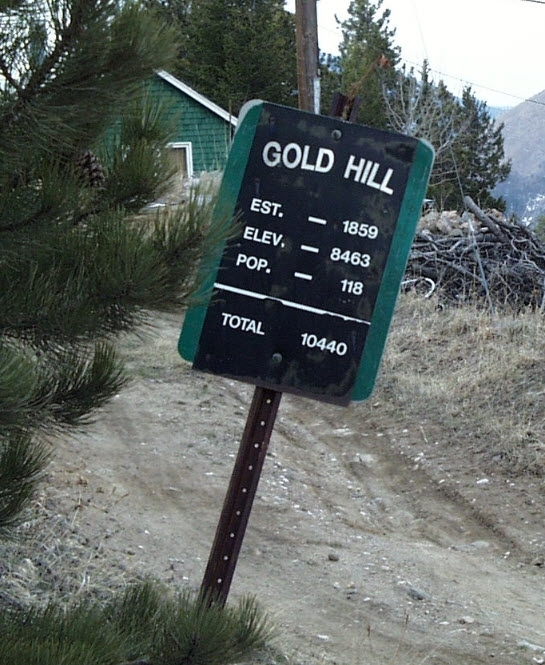
\includegraphics[width=0.4\linewidth]{type-error}\vspace{-0.5\baselineskip}
\par\end{centering}
\caption{\index{jokes}Mixing incompatible data types produces nonsensical
results.\label{fig:A-nonsensical-calculation-1}}

\end{figure}

\begin{itemize}
\item Data is \emph{immutable} (because true facts are immutable).
\item Values of different \emph{type} (population count, land area, distance,
price, location, time, growth percentage, etc.) need to be handled
separately. For example, it is an error to add a distance to a population
count.
\item Data processing should be performed according to \emph{mathematical
formulas}. True mathematical formulas are immutable and always give
the same results from the same input data.
\end{itemize}
Violating these tenets produces nonsense (see Fig.\ \ref{fig:A-nonsensical-calculation-1}
for a real-life illustration).

The power of the principles of mathematics extends over all epochs
and all cultures; math is the same in San Francisco, in Rio de Janeiro,
in Kuala-Lumpur, and in Pyongyang (Fig.\ \ref{fig:The-Pyongyang-method-of-error-free-programming-1}).

\addsec{Functional programming is math}

The functional programming paradigm is based on mathematical principles:
values are immutable, data processing is coded through formula-like
expressions, and each type of data is required to match correctly
during the computations. The type-checking process automatically prevents
programmers from making many kinds of coding errors. In addition,
programming languages such as Scala and Haskell have a set of features
adapted to building powerful abstractions and domain-specific languages.
This power of abstraction is not accidental. Since mathematics is
the ultimate art of building abstractions, math-based functional programming
languages capitalize on several millennia of mathematical experience.

A prominent example of how mathematics informs the design of programming
languages is the connection between constructive logic\footnote{\texttt{\href{https://en.wikipedia.org/wiki/Intuitionistic_logic}{https://en.wikipedia.org/wiki/Intuitionistic\_logic}}}
and the programming language\textsf{'}s type system, called the Curry-Howard
(CH) correspondence. The main idea of the CH correspondence\index{Curry-Howard correspondence}
is to think of programs as mathematical formulas that compute a value
of a certain type $A$. The CH correspondence is between programs
and logical propositions: To any program that computes a value of
type $A$, there corresponds a proposition stating that \textsf{``}a value
of type $A$ can be computed\textsf{''}.

This may sound rather theoretical so far. To see the real value of
the CH correspondence, recall that formal logic has operations \textsf{``}\textbf{\emph{and}}\textsf{''},
\textsf{``}\textbf{\emph{or}}\textsf{''}, and \textsf{``}\textbf{\emph{implies}}\textsf{''}. For any
two propositions $A$, $B$, we can construct the propositions \textsf{``}$A$
\textbf{\emph{and}} $B$\textsf{''}, \textsf{``}$A$ \textbf{\emph{or}} $B$\textsf{''}, \textsf{``}$A$
\textbf{\emph{implies}} $B$\textsf{''}. These three logical operations are
foundational; without one of them, the logic is \emph{incomplete}
(cannot derive some theorems).

A programming language \textbf{obeys the CH correspondence}\index{Curry-Howard correspondence}
with the logic if for any types $A$, $B$, the language also contains
composite types corresponding to the logical formulas \textsf{``}$A$ \textbf{\emph{or}}
$B$\textsf{''}, \textsf{``}$A$ \textbf{\emph{and}} $B$\textsf{''}, \textsf{``}$A$ \textbf{\emph{implies}}
$B$\textsf{''}. In Scala, these composite types are \lstinline!Either[A, B]!,
the tuple \lstinline!(A, B)!, and the function type \lstinline!A => B!.
All modern functional languages such as OCaml, Haskell, Scala, F\#,
and Swift support these three type constructions and thus obey the
CH correspondence. Having a \emph{complete} logic in a language\textsf{'}s
type system enables declarative domain-driven code design.\footnote{\texttt{\href{https://fsharpforfunandprofit.com/ddd/}{https://fsharpforfunandprofit.com/ddd/}}}

\begin{wrapfigure}{I}{0.5\columnwidth}%
\begin{centering}
\vspace{-0.5\baselineskip}
\par\end{centering}
\vspace{-3\baselineskip}
\end{wrapfigure}%

\begin{figure}

\begin{centering}

\includegraphics[width=0.5\linewidth]{no-bugs}
\par\end{centering}
\caption{\index{jokes}The Pyongyang method of error-free software engineering.\label{fig:The-Pyongyang-method-of-error-free-programming-1}}

\end{figure}

It is interesting to note that most older programming languages (C/C++,
Java, JavaScript, Python) do not support some of these composite types.
In other words, these programming languages have type systems based
on an incomplete logic. As a result, users of these languages have
to implement burdensome workarounds that make for error-prone code.
Failure to follow mathematical principles has real costs (Figure~\ref{fig:The-Pyongyang-method-of-error-free-programming-1}).

\addsec{The power of abstraction}

Early adopters of Scala, such as Netflix, LinkedIn, and Twitter, were
implementing what is now called \textsf{``}big data engineering\textsf{''}. The required
software needs to be highly concurrent, distributed, and resilient
to failure. Those software companies used Scala as their main implementation
language and reaped the benefits of functional programming.

What makes Scala suitable for big data tasks? The only reliable way
of managing massively concurrent code is to use sufficiently high-level
abstractions that make application code declarative. The two most
important such abstractions are the \textsf{``}resilient distributed dataset\textsf{''}
(RDD) of Apache Spark and the \textsf{``}reactive stream\textsf{''} used in systems
such as Kafka, Akka Streams, and Apache Flink. While these abstractions
are certainly implementable in Java or Python, a fully declarative
and type-safe usage is possible only in a programming language with
a sophisticated type system. Among the currently available mature
functional languages, only Scala and Haskell are technically adequate
for that task, due to their support for typeclasses and higher-order
types. The early adopters of Scala were able to benefit from the powerful
abstractions Scala supports. In this way, Scala enabled those businesses
to engineer and to scale up their massively concurrent computations.

It remains to see why Scala (and not, say, OCaml or Haskell) became
the \emph{lingua franca} of big data.

\addsec{Scala is Java on math }

The recently invented general-purpose functional programming languages
may be divided into \textsf{``}academic\textsf{''} (OCaml, Haskell) and \textsf{``}industrial\textsf{''}
(F\#, Scala, Swift).

The \textsf{``}academic\textsf{''} languages are clean-room implementations of well-researched
mathematical principles of programming language design (the CH correspondence
being one such principle). These languages are not limited by requirements
of compatibility with any existing platforms or libraries. Because
of this, the \textsf{``}academic\textsf{''} languages have been designed and used
for pursuing various mathematical ideas to their logical conclusion.\footnote{OCaml has recursive and polymorphic product and co-product types that
can be freely combined with object-oriented types. Haskell removes
all side effects from the language and supports type-level functions
of arbitrarily high order.} At the same time, software practitioners struggle to adopt these
programming languages due to a steep learning curve, a lack of enterprise-grade
libraries and tool support, and immature package management.

The languages from the \textsf{``}industrial\textsf{''} group are based on existing
and mature software ecosystems: F\# on .NET, Scala on JVM, and Swift
on the MacOS/iOS platform. One of the important design requirements
for these languages is 100\% binary compatibility with their \textsf{``}parent\textsf{''}
platform\textsf{'}s languages (F\# with C\#, Scala with Java, and Swift with
Objective-C). Because of this, developers can immediately take advantage
of the existing tooling, package management, and industry-strength
libraries, while slowly ramping up the idiomatic usage of new language
features. However, the same compatibility requirements dictate certain
limitations in the languages, making their design less than fully
satisfactory from the functional programming viewpoint.

It is now easy to see why the adoption rate of the \textsf{``}industrial\textsf{''}
group of languages is much higher\footnote{\texttt{\href{https://www.tiobe.com/tiobe-index/}{https://www.tiobe.com/tiobe-index/}},
archived in 2019 at \texttt{\href{http://archive.is/RsNH8}{http://archive.is/RsNH8}}} than that of the \textsf{``}academic\textsf{''} languages. The transition to the
functional paradigm is also smoother for software developers because
F\#, Scala, and Swift seamlessly support the familiar object-oriented
programming\index{object-oriented programming} paradigm. At the same
time, these new languages still have logically complete type systems,
which gives developers an important benefit of type-safe domain modeling.

Nevertheless, the type systems of these languages are not equally
powerful. For instance, F\# and Swift are similar to OCaml in many
ways but omit OCaml\textsf{'}s parameterized modules and some other features.
Of all the mentioned languages, only Scala and Haskell directly support
typeclasses and higher-order functions on types, which are helpful
for expressing abstractions such as automatically parallelized data
sets or asynchronous data streams.

To see the impact of these advanced features, consider LINQ, a domain-specific
language for database queries on .NET, implemented in C\# and F\#
through a special built-in syntax supported by Microsoft\textsf{'}s compilers.
Analogous functionality is provided in Scala as a \emph{library},
without need to modify the Scala compiler, by several open-source
projects such as Slick and Quill. Similar libraries exist for Haskell
\textemdash{} but not in languages with less powerful type systems.

\addsec{Summary}

Only Scala has all of the features required for industrial-grade functional
programming:
\begin{enumerate}
\item Functional collections in the standard library.
\item A sophisticated type system with support for typeclasses and higher-order
types.
\item Seamless compatibility with a mature software ecosystem (JVM).
\end{enumerate}
Based on this assessment, it appears that Scala is a good choice of
an implementation language for big data engineering.
